\begin{table*}[t]
\footnotesize
\centering
\begin{tabular}{@{}cllllll@{}}
\toprule
                  & \multicolumn{3}{c}{\textbf{Seen Both Sides}}                                       & \multirow{2}{*}{\textbf{Unseen Src}} & \multirow{2}{*}{\textbf{Unseen Tgt}} & \multirow{2}{*}{\textbf{Unseen Both Sides}} \\ 
                  & \textbf{Same Direction} & \textbf{Reversed Direction} & \textbf{Unseen Direction} &                                      &                                      &                                       \\ \midrule
\textbf{8-shot ICL}   & 14.5                    & 14.5                        & 11.2                      & 13.5                                 & 13.6                                 & 14.6                                  \\
\textbf{\methodend-16}  & 15.7(+1.2)                   & 13.7(-0.8)                        & 12.6(+1.4)                      & 14.9(+1.4)                                 & 14.5(+0.9)                                 & 15.3(+0.7)                                  \\ \midrule
\textbf{\methodend-all} & 16.7                    & 16.8                        & 14.6                      & 17.6                                 & 17.0                                 & 18.4                                  \\ \bottomrule
\end{tabular}
\caption{Translation performances under  different data conditions. \methodend-16: XGLM multilingual finetuned with translation instructions on a mixture of 16 language pairs described in Section~\ref{sec:conditions}.}
\label{tab:partial}
\end{table*}

\section{Understanding the Ability of Carrying Out Translation Instructions}
In this section, we present a comprehensive analysis on how \method improves the model's ability to carry out translation instructions. 


We begin by presenting an overarching experiment where we intentionally withhold certain language pairs during the \method process, which allows us to study models' ability to carry out translation instructions under different conditions.


Furthermore, we delve deeper into our analysis by exploring how \method enhances LLMs' ability to 
carry out translation instructions from following perspectives: better understanding of translation instructions~(Section~\ref{sec:partial_scaling} and Section~\ref{sec:translation_behavior}) and better alignment between languages to execute translation instructions~(Section~\ref{sec:language_alignment}).


\subsection{Manipulating Conditions}
\label{sec:conditions}
In Section \ref{sec:finetuning}, we have presented results in a fully supervised setting, where all testing language pairs are seen during instruction tuning.  To provide further insights into LLMs' generalization ability across language pairs, we simulate a more realistic scenario where there may be a lack of source and/or target language sentences during the instruction tuning process.

More specifically, from the 13 selected languages, we hold out 6 languages as unseen languages.
We further partition the rest 7 languages into three groups: Only-Source (languages only appear on the source side), Only-Target (languages only appear on the target side) and Source-Target (languages appear on both the source and target side). We then form language pairs from these partitions following the requirement of partitions. This allows us to assess \methodend's performance under the following conditions:

\begin{itemize}
    \item \textbf{Seen Both Sides} Both the source side and target side language appear in the finetuning corpus. This can be further divided to:
        \begin{itemize}
            \item \textbf{Same Direction}. The same translation direction is trained during \methodend.
            \item \textbf{Reversed Direction}. The same translation direction does not appear when training, but the reversed direction does.
            \item \textbf{Unseen Direction}. The translation pair (neither the same nor the reverse) does not appear when training.
        \end{itemize}
    \item \textbf{Unseen Src}. Only the target language sentences appear when training.
    \item \textbf{Unseen Tgt}. Only the source language sentences appear when training.
    \item \textbf{Unseen Both Sides}. Neither source language nor target language sentences appear in the finetuning corpus.
\end{itemize}


\subsection{\method Learns to Follow Translation Instruction across Conditions}
\label{sec:partial}

We finetune XGLM on the corpus described in the previous section. Since there are 16 language directions in the training corpus, we denote the finetuned model as \methodend-16. The model finetuned on all language pairs is denoted as \methodend-all. Table~\ref{tab:partial} shows the results.  

\paragraph{\methodend-16 Brings Improvements on Most Settings, Yet Much Less Than \methodend-all.}Firstly we can see that \methodend-16 brings improvements on most settings except Reversed Direction, demonstrating the effectiveness of \methodend-16. However, the improvements are less when compared \methodend-all, even for the Same Direction partition. This can be attributed to fewer language pairs when finetuning, which we will discuss in Section \ref{sec:partial_scaling}.

\paragraph{Language Position Shift Between Training and Testing Has Negative Effects on Translation Performance.}
The translation performance of \methodend-16 on Reversed Direction degrades by 0.8 BLEU compared to 8-shot ICL. By inspecting the translation results, we find that \methodend-16 suffers from severe off-target problems, i.e. generating translations in wrong target languages. We hypothesize that this could be attributed to the shift in the relative positions of the source and target languages during training.

\paragraph{Seeing Target Languages When Finetuning is Better Than Source Languages.}
When there are unseen languages in the language direction, the improvement on Unseen Src is much larger compared to Unseen Tgt, indicating the understanding of the specified target language may be more important than the source language.

\paragraph{Unseen Both Sides Also Benefit From \method Training.} The most surprising phenomenon is that language pairs from Unseen Both Sides partition also benefit from \methodend, with an improvement of 0.7 BLEU compared to 8-shot ICL. Since \methodend-16 does not see any sentences of the source and target languages, the improvements indicate a better understanding of the translation instruction, which we will discuss in Section \ref{sec:translation_behavior}.


\begin{figure}[t]
\centering
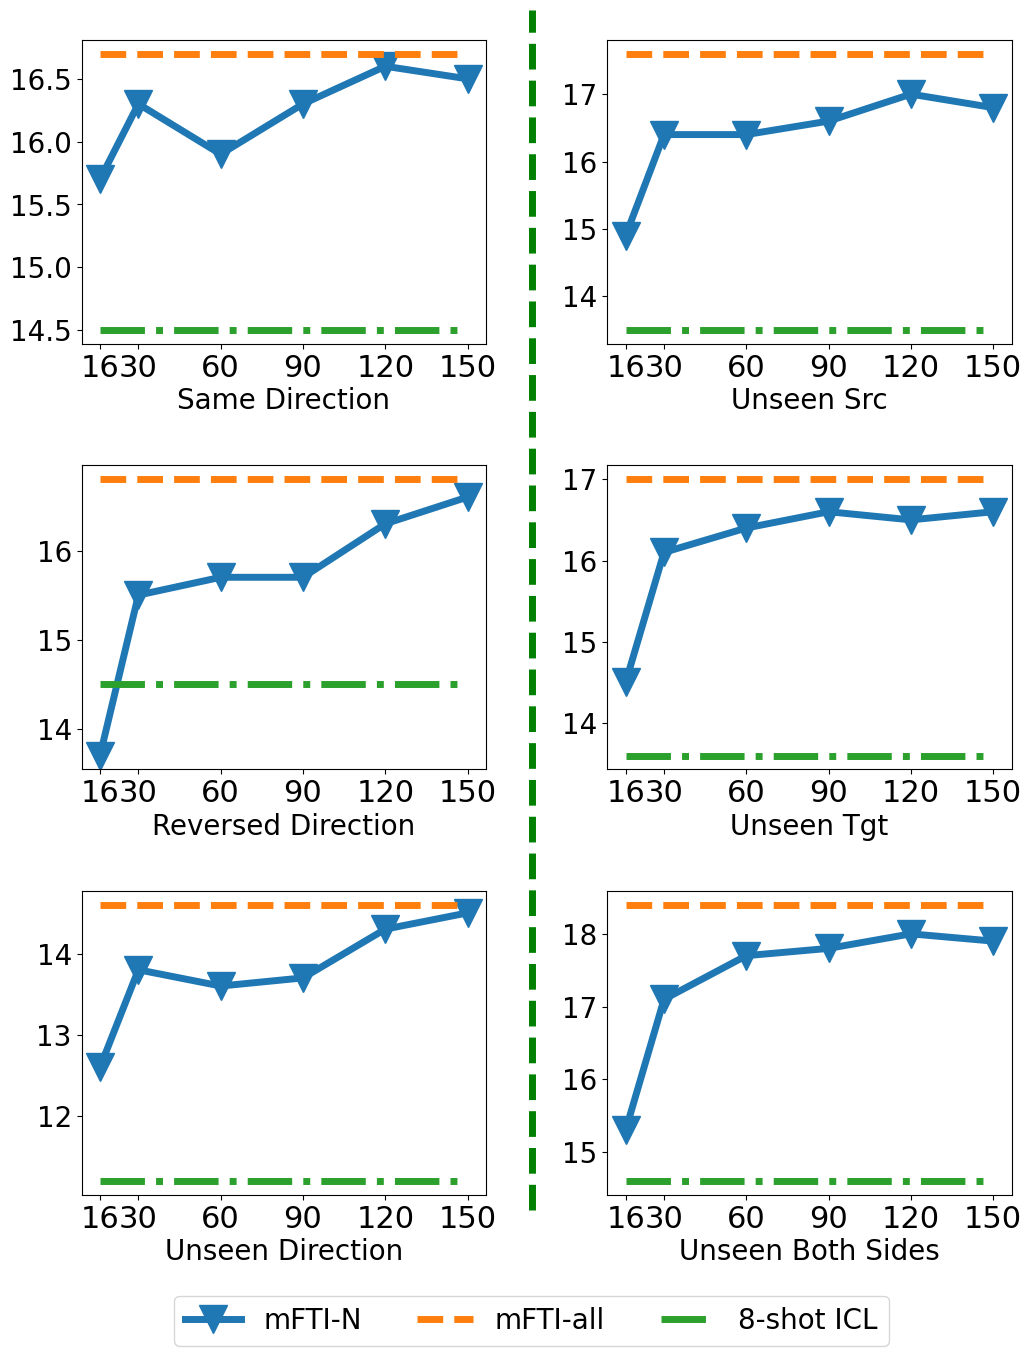
\includegraphics[width=1.0\linewidth]{figs/partial_scaling.png}
\caption{Translation performance on different partitions as the number of language pairs grows. \textit{Left}: partitions where sentences of both source and target language are seen when training. \textit{Right}: partitions where source and/or target language sentences are unseen when training. }
\label{fig:partial_scaling}
\end{figure}




\begin{figure*}[t]
\centering
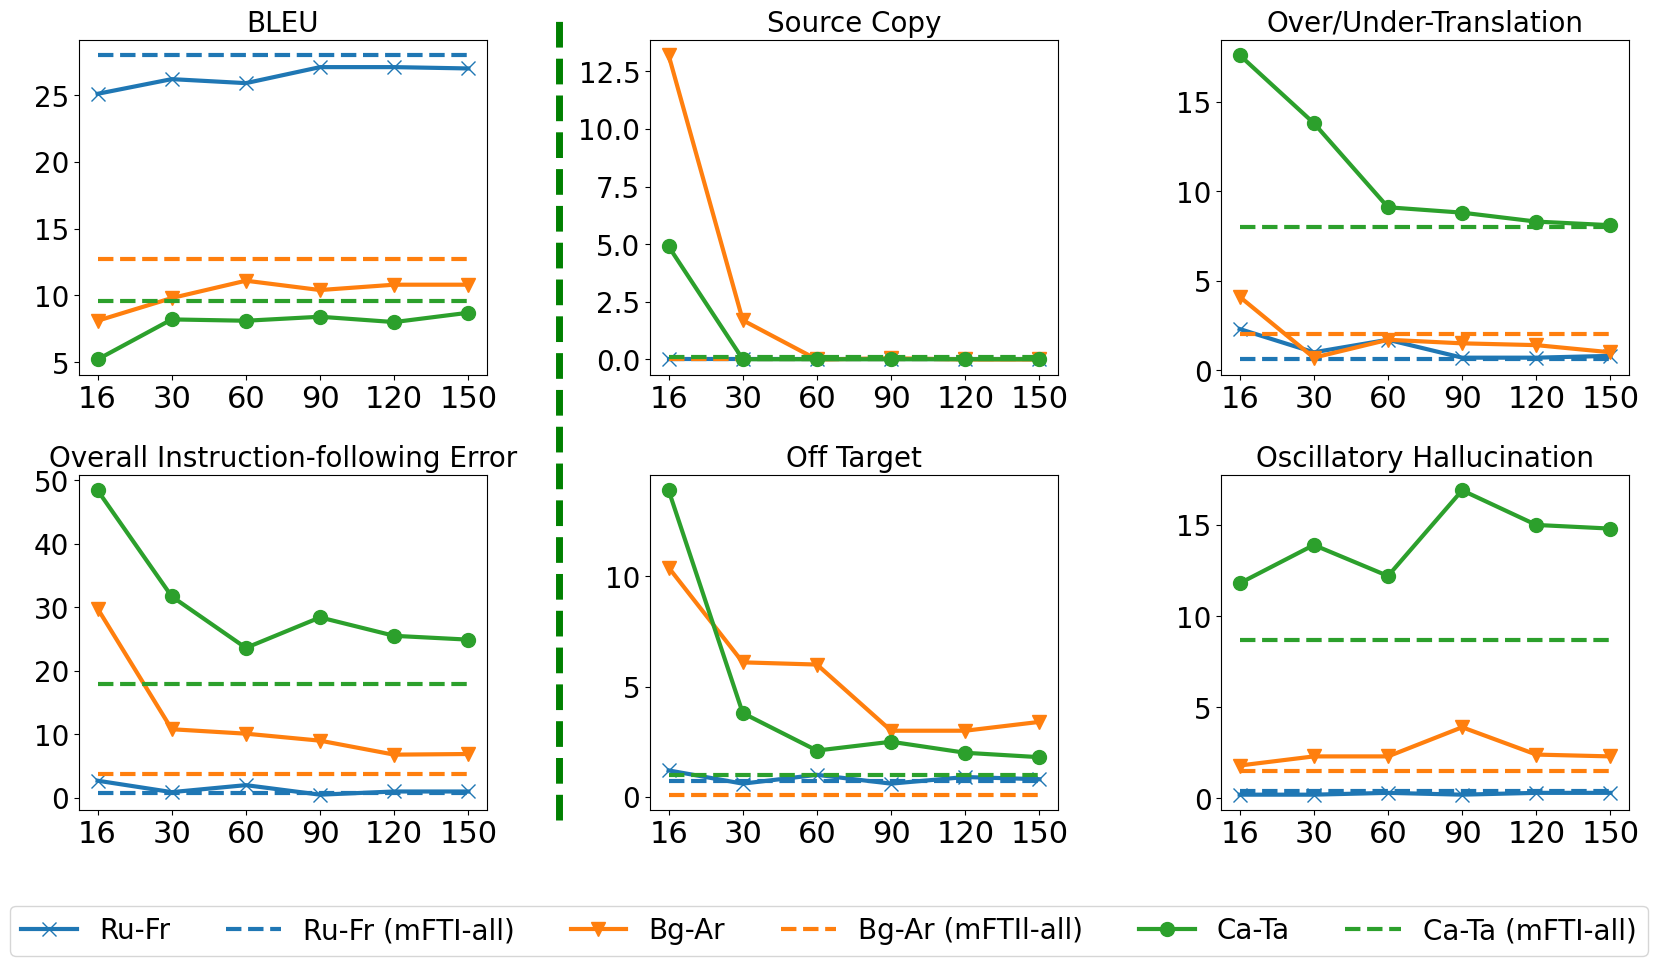
\includegraphics[width=1.0\linewidth]{figs/add_language_pairs.png}
\caption{Trends of translation and instruction-following performance on 3 Unseen-both language pairs when scaling up the number of language pairs during mFTI. The left 2 figures show the BLEU score and overall instruction-following error ratios, respectively. The rest 4 figures show the ratios of 4 specific error types, respectively, i.e. source copy, off-target, over/under translation, and oscillatory hallucination. The X-axis denotes the number of training language pairs. The Y-axis denotes the percentage of translations with specific error types.}
\label{fig:add_language_pairs}
\end{figure*}

\subsection{Instruction Tuning with More Language Pairs Leads to Better Translation Performance}
\label{sec:partial_scaling}
Previous instruction-tuning works show that scaling the number of tasks significantly benefits the unseen tasks~\citep{chung2022scaling}. Observing the performance gap of Same Direction between \methodend-16 and \methodend-all, we gradually add more language pairs to \methodend-16, and plot the translation performance on each partition in Figure~\ref{fig:partial_scaling}. In order to isolate possible effects of additional monolingual sentences, we only add language pairs that exclude the studied 13 languages~\footnote{Detailed language pairs are in Appendix \ref{appendix:Additional language}.}.

It can be seen that as the number of language pairs grows, the translation performances of all partitions generally increase, validating the importance of more language pairs. Notably, the performance of the Reversed Direction partition is significantly boosted, outperforming 8-shot ICL by a large margin when increasing the number of language pairs from 16 to 30.

Surprisingly, the performance of the Unseen Both Sides partition improves the most. Since no data of language pairs in Unseen Both Sides are added, this indicates the ability of instruction-following on these language pairs has been significantly enhanced, which we will discuss in the next section.






\subsection{\method Generalizes the Understanding of Translation Instruction to Unseen Directions}
\label{sec:translation_behavior}


In this section, we aim to understand how \method facilitates the understanding of instructions from a more fine-grained view, i.e. specific \textit{language directions} and \textit{instruction-following errors}. 

For the language directions, we select Ru$\to$Fr~(high-resource), Bg$\to$Ar~(medium-resource), Ca$\to$Ta~(low-resource) from the Unseen-Both Sides partition to study \methodend's effectiveness under different resource settings. 

For instruction errors, we identify the following four major problems in translations:




\begin{itemize}

    \item \textit{Source Copy}~(\textbf{SC}): This error occurs when the model simply copies the source sentence as the translation without making any meaningful changes. We identify this error by calculating the sentence-level BLEU score between the translations and the source sentences. If the BLEU score is above 80, it indicates that the translation is nearly identical to the source.

    \item \textit{Off-target translation}~(\textbf{OT}): In this case, the model fails to produce sentences in the target language. We detect this error by using a language identification tool, such as \textit{fasttext}, to determine the language of the generated translations.

    \item \textit{Over/under translation}~(\textbf{OU}): This error refers to situations where the model produces translations that are significantly longer or shorter than references. We consider translations with a length ratio above 2 or below 0.5 as over- or under-translations, respectively.

    \item \textit{Oscillatory hallucination}~(\textbf{OH}): This error occurs when the model gets stuck in a specific translation state and generates repeated n-grams until reaching the maximum length. We define translations with n-grams that consecutively repeat at least three times as oscillatory hallucinations.
\end{itemize}



\begin{table*}[t]
\centering
\begin{tabular}{rccccccccc}
\toprule
                       & \multicolumn{3}{c}{\textbf{Ru$\to$Fr}} & \multicolumn{3}{c}{\textbf{Bg$\to$Ar}} & \multicolumn{3}{c}{\textbf{Ca$\to$Ta}} \\ \midrule
                       & \textbf{OT$\Downarrow$}        & \textbf{OH$\Downarrow$}        & \textbf{BLEU$\Uparrow$}       & \textbf{OT$\Downarrow$}     & \textbf{OH$\Downarrow$}     & \textbf{BLEU$\Uparrow$}    & \textbf{OT$\Downarrow$}      & \textbf{OH$\Downarrow$}     & \textbf{BLEU$\Uparrow$}   \\
mFTI-16        & 1.2       & 0.2       & 25.1       & 10.4    & 1.8    & 8.1     & 13.9    & 11.8   & 5.2   \\
\textit{+ unseen-mono} & \green{0.9}       & \green{0.1}       & \green{25.4}       & \green{2.6}    & \green{0.9}    & \green{10.4}     & \green{4.4}    & \green{6.3}   & \green{6.3}    \\ \midrule
mFTI-150       & 0.8       & 0.3       & 27.0       & 3.4    & 2.3    & 10.8    & 1.8     & 14.8   & 8.7    \\
\textit{+ unseen-mono} & \green{0.7}       & \green{0.2}       & \green{27.4}       & \green{0.5}    & \green{1.5}    & \green{12.0}    & \green{1.2}     & \green{5.1}   & \green{9.3}    \\ \midrule
\methodend-all               & 0.7       & 0.2       & 28.0       & 0.1    & 1.5    & 12.7    & 1.0     & 8.7   & 9.6   \\ \bottomrule
\end{tabular}
\caption{BLEU score, off-target ratio and oscillatory hallucination ratio before and after adding monolingual sentences to the finetuning corpus. Scores where adding monolingual sentences leads to improved quality are with \green{green} background. }
\label{tab:mono}
\end{table*}

\subsubsection{Adding Irrelevant Language Pairs Reduces SC, OT and OU Ratios} 

In Section \ref{sec:partial_scaling}, we show that additional language pairs in \method lead to improved BLEU scores even for the Unseen Both Sides partition. We provide an in-depth analysis here from the aforementioned fine-grained views. We plot the trends of translation and instruction-following performance, and the ratios of 4 specific instruction-following errors as the number of additional language pairs grows. The results are in Figure~\ref{fig:add_language_pairs}.






\paragraph{More Language Pairs Reduce Instruction-Following Errors and Improve Translation Performance.}
Firstly, we can see that as more language pairs are added to the training corpus, instruction-following errors on Unseen-both language pairs are gradually reduced, leading to improvements in BLEU scores. 
Comparing different language pairs, we can see that high- and medium-resource language pairs generally perform better than low-resource language pairs on all four types of errors. Since all these language directions are unseen when instruction finetuning, it highlights the importance of language skills acquired during the pretraining phase.





\paragraph{SC: Solved.} It can be observed that after adding about 30-60 language pairs, the model learns to avoid the SC problem, indicating this is a relatively easy problem to solve.

\paragraph{OU: Decreased to the level of \methodend-all. } We can further see that adding more language pairs is also effective for reducing OU errors, as the error ratios significantly decrease as the number of language pairs grows. Notably, after scaling the number of language pairs to 150, the OU ratios of three unseen language pairs are comparable to supervised full finetuning. This demonstrates the effectiveness of \methodend.

\paragraph{OT: Decreased, but not to a satisfactory level.} Turning to the OT ratio, we observe that it also decreases as the number of language pairs grows. However, even after scaling the number of language pairs to 150, the OT ratio still cannot be decreased to the level of \methodend-all.

\paragraph{OH: No effect.} Finally, we can see that with the increment in the number of language pairs, the OH ratio does not show a clear decreasing trend, which we will further discuss in the next section.




\subsubsection{Joint Training with Monolingual Generation Instructions Helps Reduce OH and OT Problems More Efficiently}
\label{sec:mono}
In the previous section, we find that the off-target (OT) and oscillatory hallucination (OH) on some language pairs cannot be fully solved to the level of \methodend-all by adding more irrelevant language pairs. We note that both problems are only related to the target language: the OT problem can be attributed to models' inability to relate target language names to the corresponding scripts of the language, and the OH problem might be caused by the poor modeling of the target languages. We hypothesize that finetuning models on 
 instructions of monolingual generation, i.e. given a language name, generate fluent sentences from that language, should help ease these problems.

To this end, we organize the monolingual sentences of the held-out languages into monolingual generation instructions. The template we adopt is ``$[l_i]: \mathbf{y}$''. We then finetune XGLM on the dataset compromised of translation instructions and these monolingual generation instructions. 

We report the BLEU score, OT ratio and OH ratio in Table~\ref{tab:mono}.  Firstly we can see that adding monolingual generation instructions for the three Unseen Both Side language pairs can help mitigate the OT and OH problem in most scenarios, leading to better translation performance. Notably, by combining more irrelevant language pairs and monolingual sentences, the gap between \methodend-150 with monolingual sentences and \methodend-all has significantly diminished, despite that the model has never seen parallel sentences of the tested language before. 




\subsection{\method Improves Language Alignment via Pivot Languages}
\label{sec:language_alignment}




Besides the understanding of translation instruction, another crucial knowledge that models must grasp to carry out the instruction is the alignment between source and target languages. However, in scenarios where direct parallel sentences are not available, models have limited access to alignment information. This situation resembles the zero-shot setting commonly studied in multilingual translation research~\citep{gu-etal-2019-improved,zhang-etal-2020-improving,arivazhagan2019missing,liu-etal-2021-improving}. In this section, we aim to investigate the ability of \method to establish meaningful alignments through pivot languages in this scenario.


Specifically, for the three Unseen Both Sides language pairs X$\to$Y studied in the previous section, i.e. Ru$\to$Fr, Bg$\to$Ar and Ca$\to$Ta,
we start from the \methodend-150 setting, and add parallel sentences of X$\to$En and En$\to$Y to the training corpus. We then perform \method using these augmented corpora and evaluate the model's performance on test sentences that do not contain instruction-following errors. As knowledge of language alignments is the last requirement for carrying out translation instructions once the model has learned to execute translation instructions correctly, the performance on these sentences serves as a reliable indicator of the model's proficiency in language alignment.

The result is in Table~\ref{tab:pivot}. First, we can see that \methodend-150 and 8-shot ICL perform comparably, both significantly worse than \methodend-all. Since the tested three language pairs are unseen in \methodend-150, this indicates that similar to \methodend-150, the main role of ICL is to enhance the model's understanding of the translation behavior instead of source-target alignment knowledge. 
 
 However, after adding pivot parallel sentences, the model's performance (\textit{+pivot}) is significantly boosted. This demonstrates the potential of \method to leverage pivot languages to boost direct alignment between languages and improve translation performances.%

\begin{table}[t]
\centering
\begin{tabular}{rccc}
\toprule
                    & \textbf{Ru$\to$Fr} & \textbf{Bg$\to$Ar} & \textbf{Ca$\to$Ta} \\ \midrule
8-shot ICL          & 27.0           & 11.6            & 9.7                       \\
\methodend-all             & \textbf{28.2}           & \textbf{13.2}            & \underline{10.6}                       \\ \midrule
\methodend-150   & 27.5           & 11.6            & 9.2                       \\
\textit{+ pivot} & \underline{27.9}         & \underline{13.0}            & \textbf{10.8}                       \\ \bottomrule
\end{tabular}
\caption{Translation performance on test sentences without instruction-following errors. Best performances are in bold. The second-best performances are underlined.}
\label{tab:pivot}
\end{table}

